\section{A Harmonic Oscillator Potential}
%By Matt Trawick

\makelabheader %(Space for student name, etc., defined in master.tex)

\bigskip

So far, all of the potential functions we've studied have been kind of boxy-looking, with discontinuities in them.  Today we'll look at a case in which the potential energy function $U(x)$ is a continuous function.  

\begin{enumerate}[wide]

\item If the potential energy function $U(x)$ is discontinuous, what does that say about the force at the point of the discontinuity?  Is that physically reasonable?
\answerspace{0.6in}

\item Suppose that a particle is being held in place on a spring with some spring constant $\kappa$  (not to be confused with Boltzmann's constant $k$), such that the equilibrium position of the particle is $x=0$.  Sketch graphs below of $F(x)$ and $U(x)$ for the particle, and write equations for them, too.
\begin{center}
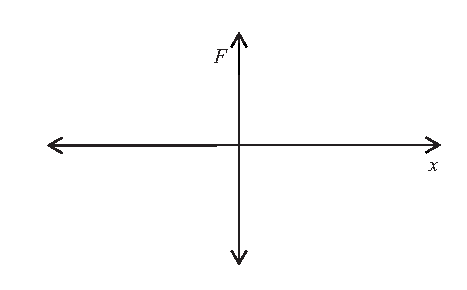
\includegraphics{harmonic_oscillator/F_axes.eps}
\includegraphics{harmonic_oscillator/U_axes.eps}
\end{center}
\bigskip

\item Think of a real world example when a small particle (say, an atom) is subject to the potential function that can be approximated by the $U(x)$ described above.  (Hint: particles on springs vibrate.  When would an atom basically be held in place, but be free to vibrate back and forth a bit?)
\answerspace{0.6in}

\item Write the time-independent Schr\"odinger equation below.  So far, all of the solutions that we've seen to the 
Schr\"odinger equation in 1-D have the form $\psi(x) = A\cos(kx)$, $\psi(x) = A\sin(kx)$, or $\psi(x) = Ae^{\pm kx}$.  Which (if any) of these functions satisfy the Schr\"odinger equation in this case?  (If you're not sure, plug them in and see.) 
\answerspace{1.6in}

\item To give yourself some sense of what $\psi(x)$ looks like for different values of energy $E$, open the following page in Firefox:
$$\verb!http://webphysics.davidson.edu/physletprob/ch10_modern/default.html!$$
Click on \button{Finite Well} on the left hand side.  In the box where the potential equation goes, type in the following: $$\verb!2500*x^2!$$
Draw sketches below of the wave functions for the three wave functions with the lowest energy, and record the energies associated with them.  
\answerspace{1.6in}

\item Are the allowed energy values and the relative spacing between them the \textit{same} as for a particle in an infinite square well, or are they \textit{different}?  Write an expression for the allowed energies $E$ in this case.
\answerspace{1.0in}

\item Look carefully at the wavefunction $\psi(x)$ for $n=18$.  For the region of $x$ where $U(x)<E$, is $\psi(x)$ a sinusoidal function?  (That is, could it be expressed in times of a single cosine or sine function?)  How can you tell whether it is or is not just by looking at the graph on the screen?  
\answerspace{1.0in}

\item Suppose that the energy of the particle were much higher (say, for n=18,000), so that the individual lobes of $\psi(x)$ were indistinguishable from each other.  Which would be greater: the probability of finding the particle near the edge of the well, or near the center of the well at $x = 0$?  How do you know?  Is this consistent with what you would expect classically, say, for an actual block of wood on a big steel spring?
\answerspace{0.8in}
\end{enumerate}
